\section{HDR ML Anomaly Challenge (Butterfly)}
{{\footnotesize
\begin{description}[labelwidth=5em, labelsep=1em, leftmargin=*, align=left, itemsep=0.3em, parsep=0em]
  \item[date:] 2025-03-03
  \item[version:] TODO
  \item[last\_updated:] 2025-03
  \item[expired:] unknown
  \item[valid:] yes
  \item[valid\_date:] TODO
  \item[url:] \href{https://www.codabench.org/competitions/3764/}{https://www.codabench.org/competitions/3764/}
  \item[doi:] TODO
  \item[domain:] Genomics; Image/CV
  \item[focus:] Detecting hybrid butterflies via image anomaly detection in genomic-informed dataset
  \item[keywords:]
    - anomaly detection
    - computer vision
    - genomics
    - butterfly hybrids
  \item[summary:] Image-based challenge for detecting butterfly hybrids in microscopy-driven species data. Participants evaluate models on Codabench using image segmentation/classification. :contentReference[oaicite:3]\{index=3\}

  \item[licensing:] TODO
  \item[task\_types:]
    - Anomaly detection
  \item[ai\_capability\_measured:]
    - Hybrid detection in biological systems
  \item[metrics:]
    - Classification accuracy
    - F1 score
  \item[models:]
    - CNN-based detectors
  \item[ml\_motif:]
    - Image/CV
  \item[type:] Dataset
  \item[ml\_task:]
    - Anomaly detection
  \item[solutions:] TODO
  \item[notes:] Hybrid detection benchmarks hosted on Codabench. :contentReference[oaicite:4]\{index=4\}

  \item[contact.name:] Imageomics/HDR Team
  \item[contact.email:] unknown
  \item[results.links.name:] ChatGPT LLM
  \item[fair.reproducible:] Yes
  \item[fair.benchmark\_ready:] Yes
  \item[ratings.software.rating:] 0
  \item[ratings.software.reason:] Not analyzed.

  \item[ratings.specification.rating:] 8.0
  \item[ratings.specification.reason:] Task of detecting rare anomalies in butterfly physics is well-described with physics motivation.

  \item[ratings.dataset.rating:] 7.0
  \item[ratings.dataset.reason:] Real detector data with injected anomalies is available, but requires NDA for full access.

  \item[ratings.metrics.rating:] 7.0
  \item[ratings.metrics.reason:] Uses ROC, F1, and anomaly precision, standard in challenge evaluations.

  \item[ratings.reference\_solution.rating:] 4.0
  \item[ratings.reference\_solution.reason:] Partial baselines described, but no codebase or reproducible runs.

  \item[ratings.documentation.rating:] 6.0
  \item[ratings.documentation.reason:] Challenge site includes overview and metrics, but limited in walkthrough or examples.

  \item[id:] hdr\_ml\_anomaly\_challenge\_butterfly
  \item[Citations:] \cite{campolongo2025buildingmachinelearningchallenges}
  \item[Ratings:]
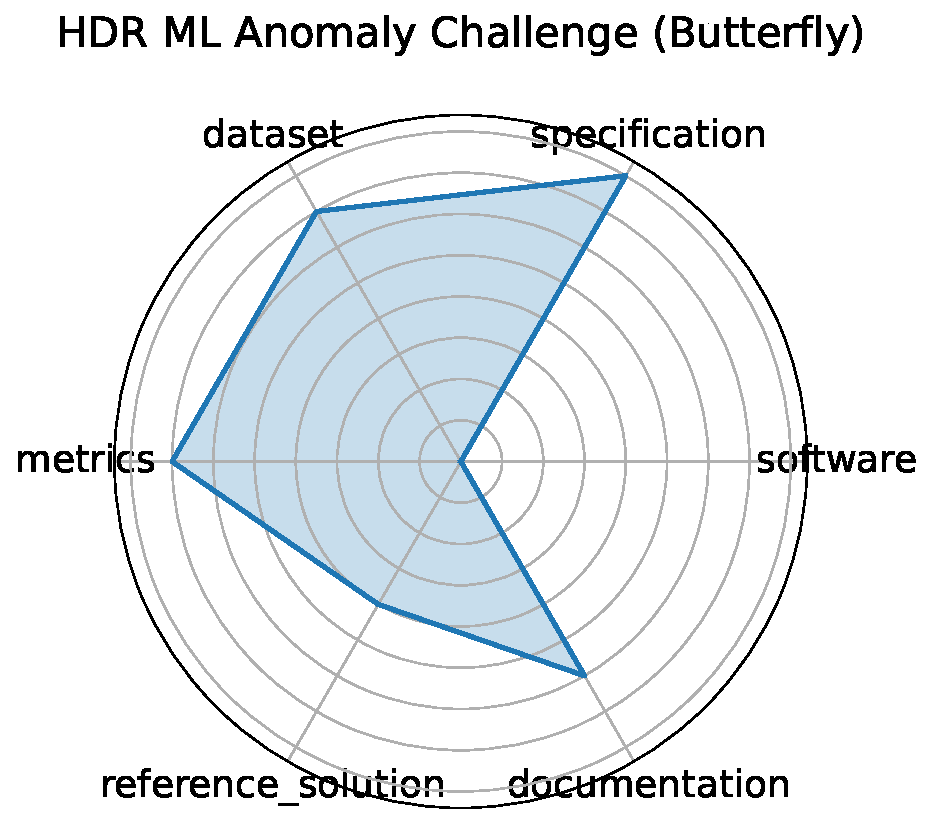
\includegraphics[width=0.2\textwidth]{hdr_ml_anomaly_challenge_butterfly_radar.pdf}
\end{description}
}}
\clearpage